\subsection{Parte (a): Descrição do Diagrama de Blocos}

\begin{figure}[H]
    \centering
    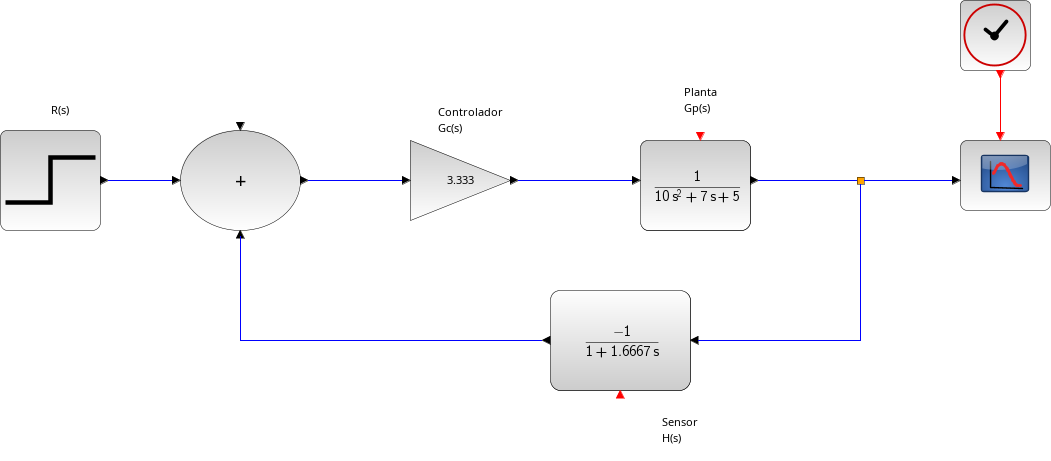
\includegraphics[width=0.8\textwidth]{atividades/4-atividade/assets/diagrama-blocos.png}
    \caption{Diagrama de blocos do sistema de controle proporcional.}
    \label{fig:diagrama_blocos}
\end{figure}

O diagrama de blocos apresentado na Figura~\ref{fig:diagrama_blocos} ilustra a configuração do sistema de controle:

\begin{itemize}
    \item \textbf{Controlador Proporcional (\(G_c(s)\))}: Com ganho de \(\frac{10}{3}\) = (\(3.333\)), o controlador ajusta a saída com base na diferença entre a referência e o sinal medido pelo sensor.
    \item \textbf{Planta (\(G_p(s)\))}: Representada pela função de transferência \(\frac{1}{10s^2 + 7s + 5}\), que descreve a dinâmica do sistema massa-mola-amortecedor.
    \item \textbf{Sensor (\(H(s)\))}: O sensor é modelado como um sistema de primeira ordem com a função de transferência \(\frac{1}{1 + 1.6667s}\), capturando a resposta da variável controlada com uma certa constante de tempo.
    \item \textbf{Soma (\(\Sigma\))}: Um somador que computa a diferença entre a referência e a saída do sensor, alimentando essa diferença para o controlador.
    \item \textbf{Realimentação}: O loop de realimentação é crucial para garantir que a saída do sistema esteja em conformidade com a entrada desejada.
\end{itemize}

O sistema é projetado para monitorar e ajustar a saída de modo a atingir um estado desejado, com foco na estabilidade e eficiência do controle.

